\documentclass[aspectratio=169]{beamer}

% ════════════════════════════════════════════════════════════════
% THEME FOUNDATION
% ════════════════════════════════════════════════════════════════
\usetheme{default}
\setbeamertemplate{navigation symbols}{}
\setbeamersize{text margin left=0.8cm, text margin right=0.8cm}

% ─── COLOR PALETTE ───────────────────────────────────────────
\definecolor{midnightblue}{RGB}{12, 44, 88}
\definecolor{royalblue}{RGB}{28, 88, 160}
\definecolor{warmorange}{RGB}{240, 108, 20}
\definecolor{softgreen}{RGB}{15, 140, 70}
\definecolor{codered}{RGB}{180, 28, 28}
\definecolor{lavender}{RGB}{100, 80, 200}
\definecolor{lightbg}{RGB}{247, 249, 255}
\definecolor{accentyellow}{RGB}{255, 200, 30}

\setbeamercolor{background canvas}{bg=lightbg}
\setbeamercolor{frametitle}{bg=midnightblue, fg=white}
\setbeamercolor{structure}{fg=royalblue}
\setbeamercolor{item}{fg=warmorange}
\setbeamercolor{subitem}{fg=royalblue}
\setbeamercolor{block title}{bg=royalblue, fg=white}
\setbeamercolor{block body}{bg=royalblue!8, fg=midnightblue}
\setbeamercolor{alerted text}{fg=warmorange}
\setbeamercolor{example text}{fg=softgreen}
\setbeamercolor{normal text}{fg=midnightblue}
\setbeamerfont{frametitle}{series=\bfseries, size=\large}

% ─── FRAME TITLE BAR (slide number only: single-pass compile) ─
\setbeamertemplate{frametitle}{%
  \nointerlineskip
  \begin{beamercolorbox}[wd=\paperwidth, ht=0.6cm, dp=0.2cm, leftskip=0.5cm]{frametitle}
    \usebeamerfont{frametitle}\insertframetitle
    \hfill{\footnotesize\color{white!70}\insertframenumber\hspace{0.4cm}}
  \end{beamercolorbox}%
  \begin{beamercolorbox}[wd=\paperwidth, ht=0.06cm]{frametitle}
    \color{warmorange}\rule{\paperwidth}{0.06cm}
  \end{beamercolorbox}%
  \vskip2mm}

\setbeamertemplate{itemize item}{\color{warmorange}\textbf{$\blacktriangleright$}}
\setbeamertemplate{itemize subitem}{\color{royalblue}$\triangleright$}

% ════════════════════════════════════════════════════════════════
% PACKAGES (kept minimal for fast compiles)
% ════════════════════════════════════════════════════════════════
\usepackage[utf8]{inputenc}
\usepackage[T1]{fontenc}
\usepackage[sfdefault]{FiraSans}
\usepackage{FiraMono}
\usepackage[expansion=false]{microtype}
\usepackage{booktabs}
\usepackage{tikz}
\usetikzlibrary{arrows.meta, positioning}
\usepackage{listings}
\usepackage{tcolorbox}
\tcbuselibrary{skins}
\usepackage{soul}
\usepackage[normalem]{ulem}

% ─── LISTINGS STYLE ──────────────────────────────────────────
\lstset{
  basicstyle=\ttfamily\footnotesize,
  backgroundcolor=\color{midnightblue!6},
  frame=single, framerule=0pt,
  rulecolor=\color{royalblue!30},
  keywordstyle=\color{royalblue}\bfseries,
  commentstyle=\color{softgreen},
  stringstyle=\color{codered!80},
  showstringspaces=false, breaklines=true,
  columns=fullflexible, keepspaces=true
}

% ════════════════════════════════════════════════════════════════
% CALLOUT BOXES
% ════════════════════════════════════════════════════════════════
\newtcolorbox{funfact}{
  enhanced, colback=accentyellow!18, colframe=warmorange!80,
  fonttitle=\bfseries\small\color{midnightblue},
  title={$\bigstar$\ \ Fun Fact}, fontupper=\small,
  arc=6pt, boxrule=1.2pt, left=5pt, right=5pt, top=3pt, bottom=3pt
}
\newtcolorbox{protip}{
  enhanced, colback=softgreen!10, colframe=softgreen!70,
  fonttitle=\bfseries\small, title={$\checkmark$\ \ Pro Tip}, fontupper=\small,
  arc=6pt, boxrule=1.2pt, left=5pt, right=5pt, top=3pt, bottom=3pt
}
\newtcolorbox{warnbox}{
  enhanced, colback=codered!6, colframe=codered!70,
  fonttitle=\bfseries\small, title={$\times$\ \ Common Mistake}, fontupper=\small,
  arc=6pt, boxrule=1.2pt, left=5pt, right=5pt, top=3pt, bottom=3pt
}
\newtcolorbox{quip}{
  enhanced, colback=lavender!12, colframe=lavender!60,
  arc=6pt, boxrule=0.8pt, left=6pt, right=6pt, top=4pt, bottom=4pt,
  fontupper=\small\itshape\color{midnightblue!90}
}
\newtcolorbox{errorlog}{
  enhanced, colback=codered!6, colframe=codered!60,
  fonttitle=\bfseries\small, coltitle=white, colbacktitle=codered!80,
  title={$\times$\ Overleaf Error Log (do not panic!)},
  arc=6pt, boxrule=1pt, left=5pt, right=5pt, top=3pt, bottom=3pt,
  fontupper=\ttfamily\scriptsize\color{codered!80}
}
\newtcolorbox{cheatcode}{
  enhanced, colback=midnightblue!8, colframe=royalblue!60,
  fonttitle=\bfseries\small, title={$\Rightarrow$\ \ Cheat Code}, fontupper=\small,
  arc=6pt, boxrule=1pt, left=5pt, right=5pt, top=3pt, bottom=3pt
}
% infobox{colour}{title}: generic titled card
\newtcolorbox{infobox}[2]{
  enhanced, colback=#1!8, colframe=#1!80!black, boxrule=0.8pt, arc=4pt,
  fonttitle=\bfseries\small, title={#2}, fontupper=\small,
  left=4pt, right=4pt, top=2pt, bottom=2pt
}

% ─── TikZ STYLES ─────────────────────────────────────────────
\tikzset{
  startstop/.style={rectangle, rounded corners, minimum width=1.7cm,
    minimum height=0.6cm, text centered, draw=black, fill=red!30, font=\small},
  process/.style={rectangle, minimum width=1.7cm, minimum height=0.6cm,
    text centered, draw=black, fill=orange!30, font=\small},
  arrow/.style={thick, ->, >=Stealth},
  chip/.style={rounded corners=3pt, draw=#1!70!black, fill=#1!12,
    minimum width=3.3cm, minimum height=1.2cm, text width=3.1cm, align=center}
}

% ─── DEMO-TIME SLIDE: \demoslide{colour}{subtitle}{tagline}{presenter cues}
\newcommand{\demoslide}[4]{%
  {\colorlet{demobg}{#1}%
   \setbeamertemplate{background canvas}{%
     \begin{tikzpicture}
       \useasboundingbox (0,0) rectangle (\the\paperwidth,\the\paperheight);
       \fill[demobg] (0,0) rectangle (\the\paperwidth,\the\paperheight);
       \fill[white, opacity=0.07] (\the\paperwidth,\the\paperheight) -- ++(-6,0) -- ++(6,-9) -- cycle;
       \fill[warmorange, opacity=0.9] (0,0) rectangle (\the\paperwidth,0.35);
     \end{tikzpicture}}%
   \begin{frame}[plain]
     \begin{center}
       {\color{white}\fontsize{40}{48}\selectfont\ttfamily\bfseries DEMO TIME}\\[0.3cm]
       {\color{accentyellow}\fontsize{20}{26}\selectfont #2}\\[0.2cm]
       {\color{white!75}\normalsize #3}\\[0.5cm]
       \begin{tcolorbox}[enhanced, colback=black!70, colframe=accentyellow,
           arc=6pt, boxrule=1.2pt, width=0.8\textwidth,
           center, halign=center, fontupper=\small\color{white}]
         #4
       \end{tcolorbox}
     \end{center}
   \end{frame}}}

% ─── Diagram-gallery chip: \chip{x}{y}{colour}{title}{examples}
\newcommand{\chip}[5]{\node[chip=#3] at (#1,#2)
  {{\footnotesize\bfseries #4}\\[-1pt]{\scriptsize #5}};}

% ─── TITLE INFO ──────────────────────────────────────────────
\title[Mastering \LaTeX]{The End of Formatting Nightmares}
\subtitle{Mastering \LaTeX\ \& Overleaf for Professional Automation}
\author{\textbf{Abel Thomas Anil}}
\date{17/10/2026}

\begin{document}

% ═══ 1 — TITLE ═══════════════════════════════════════════════
{\setbeamertemplate{background canvas}{%
  
\begin{tikzpicture}
    \useasboundingbox (0,0) rectangle (\the\paperwidth,\the\paperheight);
    \fill[midnightblue] (0,0) rectangle (\the\paperwidth,\the\paperheight);
    \fill[warmorange, opacity=0.85] (\the\paperwidth,0) -- ++(-4.5,0)
      -- (\the\paperwidth,\the\paperheight) -- cycle;
    \fill[royalblue, opacity=0.5] (\the\paperwidth,0) -- ++(-7,0) -- ++(7,5) -- cycle;
    \draw[warmorange!60, line width=3pt] (0,\the\paperheight) ++(1,-0.9)
      -- ++(-0.7,0) -- ++(0,-1.4);
    \draw[royalblue!80, line width=3pt] (0,0) ++(1,0.9) -- ++(-0.7,0) -- ++(0,1.4);
  \end{tikzpicture}}
\begin{frame}[plain]
  \begin{center}
    {\color{white}\fontsize{24}{30}\selectfont\bfseries The End of Formatting Nightmares}\\[0.4cm]
    {\color{warmorange}\rule{6cm}{0.5pt}}\\[0.4cm]
    {\color{white!85}\large Mastering \LaTeX\ \& Overleaf for Professional Automation}\\[0.7cm]
    {\color{warmorange}\Large\textbf{Abel Thomas Anil}}\\[0.2cm]
    {\color{white!60}\small 17/10/2026}
  \end{center}
\end{frame}}

% ═══ 2 — ROADMAP ═════════════════════════════════════════════
\begin{frame}[c]{Today's Roadmap}
  \centering
  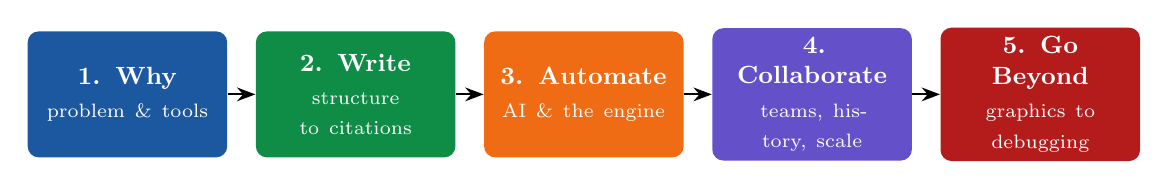
\begin{tikzpicture}[node distance=3.5mm,
    act/.style={rounded corners=4pt, minimum width=2.5cm, minimum height=1.6cm,
      text width=2.3cm, align=center, text=white, font=\small\bfseries}]
    \node[act, fill=royalblue] (a) {\hyphenpenalty=10000 \exhyphenpenalty=10000
      1. Why\\[1pt]{\scriptsize\mdseries problem \& tools}};
    \node[act, fill=softgreen, right=of a] (b) {\hyphenpenalty=10000 \exhyphenpenalty=10000
      2. Write\\[1pt]{\scriptsize\mdseries structure to citations}};
    \node[act, fill=warmorange, right=of b] (c) {\hyphenpenalty=10000 \exhyphenpenalty=10000
      3. Automate\\[1pt]{\scriptsize\mdseries AI \& the engine}};
    \node[act, fill=lavender, right=of c] (d) {\hyphenpenalty=10000 \exhyphenpenalty=10000
      4. Collaborate\\[1pt]{\scriptsize\mdseries teams, history, scale}};
    \node[act, fill=codered, right=of d] (e) {\hyphenpenalty=10000 \exhyphenpenalty=10000
      5. Go Beyond\\[1pt]{\scriptsize\mdseries graphics to debugging}};
    \foreach \p/\q in {a/b, b/c, c/d, d/e} \draw[arrow] (\p) -- (\q);
  \end{tikzpicture}
\end{frame}

% ═══ 3 — THE PROBLEM ═════════════════════════════════════════
\begin{frame}{We've All Been Here...}
  \begin{columns}[c]
    \column{0.6\textwidth}
      \begin{itemize}
        \item It feels like 40\% writing...
        \item ...and 60\% fighting margins, fonts, and floating images.
        \item Numbering figures by hand? Updating a TOC (Table of Contents) manually?
        \item In MS (Microsoft) Word, nudging one image by 1\,mm can wreck the page.
      \end{itemize}
      \vspace{0.3cm}
      \begin{quip}
        ``It's 2026. We shouldn't be dragging images around with a mouse and hoping for the best.''
      \end{quip}
    \column{0.38\textwidth}
      \begin{center}
      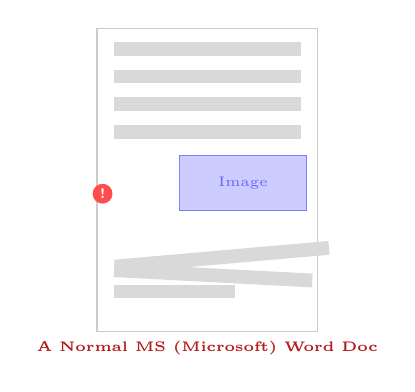
\begin{tikzpicture}[scale=0.7]
        \fill[white, draw=gray!40, line width=0.5pt] (0,0) rectangle (4,5.5);
        \foreach \y in {5, 4.5, 4, 3.5} {
          \fill[gray!30] (0.3,\y) rectangle (3.7,\y+0.25);
        }
        \fill[blue!20, draw=blue!50] (1.5,2.2) rectangle (3.8,3.2);
        \node[font=\tiny, text=blue!60] at (2.65,2.7) {Image};
        \fill[red!70] (0.1,2.5) circle (0.18);
        \node[font=\tiny\bfseries, text=white] at (0.1,2.5) {!};
        \fill[gray!30, rotate around={5:(2,1.5)}] (0.3,1.2) rectangle (4.2,1.45);
        \fill[gray!30, rotate around={-3:(2,0.9)}] (0.3,0.9) rectangle (3.9,1.15);
        \fill[gray!30] (0.3,0.6) rectangle (2.5,0.85);
        \node[font=\tiny\bfseries, text=codered] at (2,-.3) {A Normal MS (Microsoft) Word Doc};
      \end{tikzpicture}
      \end{center}
  \end{columns}
\end{frame}

% ═══ 4 — THE PARADIGM SHIFT ══════════════════════════════════
\begin{frame}[fragile]{Code Your Documents}
  \begin{columns}[c]
    \column{0.48\textwidth}
      \textbf{\color{midnightblue}You Write:}
      \vspace{0.2cm}
      \begin{lstlisting}[language=TeX]
\section{Introduction}
This is my \textbf{report}.
\begin{equation}
  E = mc^2
\end{equation}
      \end{lstlisting}
    \column{0.48\textwidth}
      \textbf{\color{midnightblue}\LaTeX\ Produces:}
      \vspace{0.2cm}

      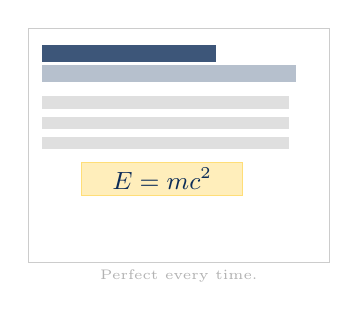
\begin{tikzpicture}[scale=0.85]
        \fill[white, draw=gray!40] (0,0) rectangle (4.5,3.5);
        \fill[midnightblue!80] (0.2,3.0) rectangle (2.8,3.25);
        \fill[midnightblue!30] (0.2,2.7) rectangle (4,2.95);
        \foreach \y in {2.3, 2.0, 1.7} {
          \fill[gray!25] (0.2,\y) rectangle (3.9,\y+0.18);
        }
        \fill[accentyellow!30, draw=accentyellow!60] (0.8,1.0) rectangle (3.2,1.5);
        \node[font=\small, text=midnightblue] at (2,1.25) {$E = mc^2$};
        \node[font=\tiny, text=gray!60] at (2.25,-0.2) {Perfect every time.};
      \end{tikzpicture}
  \end{columns}
  \vspace{0.3cm}
  \begin{funfact}
    Donald Knuth created \TeX\ in 1978 because he was appalled by how ugly the typeset proofs
    of his own book looked. Leslie Lamport later built \LaTeX\ on top of it.
  \end{funfact}
\end{frame}

% ═══ 5 — MEET THE TOOLS ══════════════════════════════════════
\begin{frame}{Meet the Tools: \LaTeX\ + Overleaf}
  \begin{columns}[T]
    \column{0.48\textwidth}
      \begin{infobox}{royalblue}{\LaTeX\ (``Lay-tech'')}
        A markup language for documents. You write content with structural commands, and the
        compiler produces a cleanly formatted PDF (Portable Document Format).
      \end{infobox}
    \column{0.48\textwidth}
      \begin{infobox}{softgreen}{Overleaf}
        ``Google Docs for \LaTeX'': runs in your browser, shows the PDF next to your source,
        and supports real-time collaboration.
      \end{infobox}
  \end{columns}
  \vspace{0.3cm}
  \centering\footnotesize
  \begin{tabular}{@{}p{2.5cm}p{5.2cm}p{5.2cm}@{}}
    \toprule
    \textbf{Aspect} & \textbf{Word processor} & \textbf{\LaTeX} \\
    \midrule
    Editing model & What you see is what you get & Write markup, then compile it \\
    Mathematics & Equation editor, limited control & Native, publication-grade \\
    Cross-references & Manual or semi-automatic & Automatic via \texttt{\textbackslash label}, \texttt{\textbackslash ref} \\
    Version control & Awkward, binary files & Plain text, Git-friendly \\
    \bottomrule
  \end{tabular}
\end{frame}

% ═══ 6 — DEMO: INTERFACE ═════════════════════════════════════
\demoslide{royalblue}{The Interface}{Let's Look at the Engine}{%
  Open the \texttt{sample project} in Overleaf\\[0.15cm]
  \textbf{\color{accentyellow}Point out:} file tree $\cdot$ source editor $\cdot$ PDF preview\\
  Recompile button $\cdot$ Logs panel $\cdot$ Visual Editor toggle}

% ═══ 7 — ANATOMY ═════════════════════════════════════════════
\begin{frame}[fragile]{Anatomy of a Document}
  \begin{columns}[T]
    \column{0.5\textwidth}
      \begin{lstlisting}[language=TeX]
\documentclass{article}
\usepackage{graphicx}  % preamble

\begin{document}       % body starts
\section{Introduction}
Hello world! This is my
first \textbf{bold} statement.
\end{document}
      \end{lstlisting}
    \column{0.46\textwidth}
      \begin{infobox}{royalblue}{1. The Preamble}
        Document class and packages: the setup area above
        \texttt{\textbackslash begin\{document\}}.
      \end{infobox}
      \vspace{0.1cm}
      \begin{infobox}{softgreen}{2. The Body}
        Your content, between \texttt{\textbackslash begin\{document\}} and
        \texttt{\textbackslash end\{document\}}.
      \end{infobox}
      \vspace{0.15cm}
      {\footnotesize\textbf{Classes:} \texttt{article} $\cdot$ \texttt{report} $\cdot$
      \texttt{book} $\cdot$ \texttt{beamer} $\cdot$ \texttt{IEEEtran}}
  \end{columns}
\end{frame}

% ═══ 8 — TEMPLATES ═══════════════════════════════════════════
\begin{frame}{Stand on the Shoulders of Giants}
  \begin{itemize}
    \item You \textbf{never} start from scratch.
    \item Overleaf has thousands of publisher, thesis, CV and poster templates.
    \item Change one line: \texttt{\textbackslash documentclass\{IEEEtran\}}
    \item Your content stays; the layout follows the template.
  \end{itemize}
  \vspace{0.3cm}
  \begin{columns}[T]
    \column{0.5\textwidth}
      \begin{block}{Template families}
        \small
        IEEE (Institute of Electrical and Electronics Engineers)\\
        ACM (Association for Computing Machinery)\\
        Nature $\cdot$ Springer $\cdot$ University theses\\
        CVs (Curriculum Vitae) $\cdot$ Posters $\cdot$ Presentations
      \end{block}
    \column{0.45\textwidth}
      \begin{protip}
        Open Overleaf $\to$ New Project $\to$ From Template.
        Search ``IEEE'' and start writing.
      \end{protip}
  \end{columns}
\end{frame}

% ═══ 9 — EVERYDAY COMMANDS ═══════════════════════════════════
\begin{frame}[fragile]{Everyday Commands}
  \begin{columns}[T]
    \column{0.52\textwidth}
      \begin{itemize}\small
        \item Styles: \verb|\textbf{}| \verb|\textit{}| \verb|\emph{}| \verb|\texttt{}|
        \item Sizes: \verb|\small| \verb|\large| \verb|\Huge|
        \item Structure: \verb|\section| \verb|\subsection|
        \item Blank line = new paragraph; \verb|\\| = line break
        \item Escape specials: \verb|\% \& \$ \# \_ \{ \}|
        \item Quotes: \verb|``like this''|, never the " key
      \end{itemize}
    \column{0.44\textwidth}
      \begin{lstlisting}[language=TeX]
\begin{itemize}
  \item Bullet point
\end{itemize}
\begin{enumerate}
  \item Numbered point
\end{enumerate}
      \end{lstlisting}
      \begin{protip}
        Prefer \texttt{\textbackslash emph} over \texttt{\textbackslash textit}: inside an
        italic sentence, emphasis turns upright automatically.
      \end{protip}
  \end{columns}
\end{frame}

% ═══ 10 — IMAGES & CROSS-REFERENCES ══════════════════════════
\begin{frame}[fragile]{Images and Never-Number-Anything-Again}
  \begin{columns}[T]
    \column{0.57\textwidth}
      \begin{lstlisting}[language=TeX, basicstyle=\ttfamily\scriptsize]
\begin{figure}[htbp]
  \centering
  \includegraphics[width=.8\linewidth]{photo}
  \caption{A beautiful landscape}
  \label{fig:landscape}
\end{figure}

As seen in Figure~\ref{fig:landscape},
the mountains are tall.
      \end{lstlisting}
    \column{0.4\textwidth}
      \begin{itemize}\small
        \item Add a figure on page 10, refer to it on page 2, add 5 figures before it?
          \LaTeX\ renumbers everything.
        \item \texttt{\textbackslash label} goes \emph{after} \texttt{\textbackslash caption}.
        \item \texttt{Figure\textasciitilde\textbackslash ref\{\ldots\}} keeps word and number together.
      \end{itemize}
  \end{columns}
  \vspace{0.2cm}
  \begin{funfact}
    In a 200-page thesis with 60 figures, Word means fixing each cross-reference
    \textit{individually}. In \LaTeX: hit compile, done.
  \end{funfact}
\end{frame}

% ═══ 11 — TABLES ═════════════════════════════════════════════
\begin{frame}[fragile]{Professional Tables with \texttt{booktabs}}
  \begin{columns}[T]
    \column{0.5\textwidth}
      \begin{lstlisting}[language=TeX]
\begin{tabular}{lcc}
  \toprule
  Feature & Apple & Android \\
  \midrule
  Open source & No & Mostly \\
  Price range & High & Wide \\
  \bottomrule
\end{tabular}
      \end{lstlisting}
    \column{0.46\textwidth}
      \begin{center}\small
      \begin{tabular}{lcc}
        \toprule
        Feature & Apple & Android \\
        \midrule
        Open source & No & Mostly \\
        Price range & High & Wide \\
        \bottomrule
      \end{tabular}
      \end{center}
      \begin{itemize}\small
        \item No vertical lines, just three clean rules.
        \item Columns: \texttt{l} \texttt{c} \texttt{r}; \texttt{p\{3cm\}} wraps text.
        \item \texttt{\textbackslash multicolumn} spans several columns.
      \end{itemize}
  \end{columns}
\end{frame}

% ═══ 12 — MATH ═══════════════════════════════════════════════
\begin{frame}{The Math Looks Incredible}
  \textbf{Inline math} (single dollar signs): the quadratic formula is
  $x = \frac{-b \pm \sqrt{b^2 - 4ac}}{2a}$.
  \vspace{0.2cm}

  \textbf{Display math} (Stokes' Theorem):
  \[
    \oint_C \mathbf{F} \cdot d\mathbf{r} = \iint_S (\nabla \times \mathbf{F}) \cdot d\mathbf{S}
  \]
  \begin{columns}[T]
    \column{0.48\textwidth}
      \begin{infobox}{royalblue}{Math environments}
        \texttt{equation}: numbered display. \texttt{equation*}: no number.
        \texttt{align}: lines up at \texttt{\&}. Also \texttt{cases} and \texttt{bmatrix}.
      \end{infobox}
    \column{0.48\textwidth}
      \begin{quip}
        No tiny equation-editor buttons, no hunting for the $\Sigma$ symbol. Always load
        \texttt{amsmath}.
      \end{quip}
  \end{columns}
\end{frame}

% ═══ 13 — CITATIONS ══════════════════════════════════════════
\begin{frame}[fragile]{Citations with BibTeX}
  \begin{columns}[T]
    \column{0.46\textwidth}
      \begin{enumerate}\small
        \item Create \texttt{references.bib} in your project.
        \item On Google Scholar: Cite $\to$ BibTeX, then paste the block into that file.
        \item In the text, type \texttt{\textbackslash cite\{key\}}.
      \end{enumerate}
      \small\LaTeX\ places the \texttt{[1]} and builds the References list for you.
      \vspace{0.2cm}
      \begin{protip}
        The modern alternative is \texttt{biblatex} with \texttt{biber}: more styles (APA, IEEE,
        Chicago).
      \end{protip}
    \column{0.52\textwidth}
      \begin{lstlisting}[basicstyle=\ttfamily\scriptsize]
@article{Einstein1905,
  author  = {Einstein, Albert},
  title   = {On the Electrodynamics
             of Moving Bodies},
  journal = {Annalen der Physik},
  year    = {1905}
}
% in the .tex file:
\cite{Einstein1905}
\bibliographystyle{plain}
\bibliography{references}
      \end{lstlisting}
  \end{columns}
\end{frame}

% ═══ 14 — DEMO: AUTOMATION ═══════════════════════════════════
\demoslide{softgreen!60!midnightblue}{Automation in Action}{Seeing is Believing}{%
  Open the \texttt{sample project}\\[0.15cm]
  \textbf{\color{accentyellow}Point out:} automatic TOC, list of figures and list of tables\\
  figure and table numbering $\cdot$ equations and theorems\\
  \texttt{\textbackslash cref} cross-references $\cdot$ citations resolving}

% ═══ 15 — CHEAT CODES ════════════════════════════════════════
\begin{frame}{You Don't Even Need to Memorize the Code}
  Nobody memorizes \LaTeX\ syntax anymore. Professionals \textbf{generate} it.
  \vspace{0.15cm}
  \begin{columns}[T]
    \column{0.48\textwidth}
      \begin{infobox}{royalblue}{TablesGenerator.com}
        \footnotesize Build a table visually, click Generate, copy the code.
      \end{infobox}
      \vspace{0.05cm}
      \begin{infobox}{softgreen}{Mathpix Snip}
        \footnotesize Screenshot an equation $\Rightarrow$ instant \LaTeX\ code.
      \end{infobox}
    \column{0.48\textwidth}
      \begin{infobox}{warmorange}{AI Assistants}
        \footnotesize ChatGPT, Claude or Gemini: paste the result, then verify it.
      \end{infobox}
      \vspace{0.05cm}
      \begin{infobox}{lavender}{Overleaf Visual Editor}
        \footnotesize A Word-like view for quick edits, no markup needed.
      \end{infobox}
  \end{columns}
  \vspace{0.15cm}
  \begin{cheatcode}
    \footnotesize
    ``Write me a \LaTeX\ table with 3 columns: Name, Age, Score, plus 3 sample rows.''
  \end{cheatcode}
\end{frame}

% ═══ 16 — DEMO: AI & MATH ════════════════════════════════════
\demoslide{lavender!80!midnightblue}{AI \& Math}{Let's Cheat}{%
  \textbf{\color{accentyellow}Show:} Mathpix: snip an equation $\Rightarrow$ paste the code\\
  TablesGenerator: build a table, copy it\\
  Ask an AI for a table, then fix one error together}

% ═══ 17 — PACKAGE ECOSYSTEM ══════════════════════════════════
\begin{frame}{The Package Ecosystem}
  \begin{columns}[T]
    \column{0.56\textwidth}
      \begin{itemize}\small
        \item \textbf{Full TeX Live:} thousands of CTAN (Comprehensive \TeX\ Archive Network)
          packages, ready to use.
        \item \textbf{Older TeX Live versions:} switch if an old project breaks.
        \item \textbf{Custom packages:} upload your own \texttt{.sty} files.
      \end{itemize}
      \begin{block}{Essential packages}
        \footnotesize
        \texttt{graphicx} images $\cdot$ \texttt{amsmath} equations $\cdot$ \texttt{booktabs} tables\\
        \texttt{geometry} margins $\cdot$ \texttt{xcolor} colours $\cdot$ \texttt{tikz} diagrams\\
        \texttt{listings} code $\cdot$ \texttt{hyperref} clickable links
      \end{block}
    \column{0.4\textwidth}
      \begin{funfact}
        CTAN hosts thousands of packages written by users worldwide. There is a package for
        nearly everything.
      \end{funfact}
      \vspace{0.2cm}
      \begin{warnbox}
        Load \texttt{hyperref} last (or nearly last). Loading it early can break other packages.
      \end{warnbox}
  \end{columns}
\end{frame}

% ═══ 18 — COMPILERS ══════════════════════════════════════════
\begin{frame}{Under the Hood: Compiler Engines}
  Switch engines in the Overleaf menu at any time:
  \vspace{0.1cm}
  \begin{columns}[T]
    \column{0.49\textwidth}
      \begin{infobox}{royalblue}{pdfLaTeX --- Default}
        \footnotesize Fast. Best for text, math and PNG images. Outputs PDF.
      \end{infobox}
      \vspace{0.05cm}
      \begin{infobox}{softgreen}{XeLaTeX --- Fonts}
        \footnotesize Use any system font via \texttt{fontspec}.
      \end{infobox}
    \column{0.49\textwidth}
      \begin{infobox}{lavender}{LuaLaTeX --- Advanced}
        \footnotesize Next-gen engine: Lua scripting, \texttt{fontspec}.
      \end{infobox}
      \vspace{0.05cm}
      \begin{infobox}{gray}{\LaTeX\ --- Legacy}
        \footnotesize Old route: DVI $\to$ PostScript $\to$ PDF.
      \end{infobox}
  \end{columns}
  \vspace{0.1cm}
  \begin{protip}
    \footnotesize Malayalam, Hindi or custom fonts? Use XeLaTeX or LuaLaTeX.
  \end{protip}
\end{frame}

% ═══ 19 — DEMO: THE MENU ═════════════════════════════════════
\demoslide{codered!70!midnightblue}{The Overleaf Menu}{Popping the Hood}{%
  \textbf{\color{accentyellow}Point out:} Compiler $\cdot$ TeX Live version $\cdot$ Main document\\
  Editor theme and font $\cdot$ Download source / PDF\\
  Recompile drop-down: Draft mode, Stop on first error}

% ═══ 20 — COLLABORATION ══════════════════════════════════════
\begin{frame}{Multiplayer Mode \& Review}
  \begin{itemize}
    \item \textbf{Share:} invite by email (edit or view) or send a read-only link.
    \item \textbf{Real-time co-authoring:} several cursors, one live document.
    \item \textbf{Comments and review:} margin comments, project chat, track changes
      (some features depend on your plan).
  \end{itemize}
  \vspace{0.4cm}
  \begin{quip}
    Imagine Google Docs, but instead of a DOCX file emailed back and forth as
    ``final\_v3\_REAL\_FINAL\_this\_one.docx,'' you have one live, versioned professional
    document. That's Overleaf collaboration.
  \end{quip}
\end{frame}

% ═══ 21 — INTEGRATIONS ═══════════════════════════════════════
\begin{frame}{Your Entire Workflow, Connected}
  \begin{columns}[T]
    \column{0.5\textwidth}
      \begin{infobox}{royalblue}{Reference Syncing}
        Link Zotero and Mendeley. Type \texttt{\textbackslash cite\{\}}, get a perfect bibliography.
      \end{infobox}
      \vspace{0.1cm}
      \begin{infobox}{midnightblue}{GitHub Sync}
        Treat your thesis like a software project: push and pull with Git.
      \end{infobox}
    \column{0.5\textwidth}
      \begin{infobox}{softgreen}{Journal Submission}
        Submit straight to supported publisher portals, with no reformatting.
      \end{infobox}
      \vspace{0.1cm}
      \begin{quip}
        ``Write once, submit anywhere.''
      \end{quip}
  \end{columns}
  \vspace{0.2cm}
  {\footnotesize\itshape Availability of some integrations depends on your Overleaf plan.}
\end{frame}

% ═══ 22 — VERSION HISTORY ════════════════════════════════════
\begin{frame}{Fearless Editing: The Time Machine}
  \begin{columns}[c]
    \column{0.55\textwidth}
      \begin{itemize}
        \item Browse every earlier version of your project.
        \item Roll back to 3:14 PM last Tuesday.
        \item Label milestones: ``Draft 1'', ``Sent to Prof''.
      \end{itemize}
      \vspace{0.2cm}
      \begin{funfact}
        A student once accidentally deleted their entire Chapter 4 one hour before submission.
        Version History saved them. True story (probably).
      \end{funfact}
    \column{0.42\textwidth}
      \begin{center}
      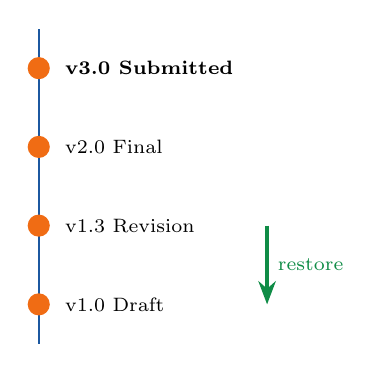
\begin{tikzpicture}[font=\scriptsize]
        \draw[royalblue, thick] (0,0) -- (0,4);
        \foreach \y/\label in {0.5/v1.0 Draft, 1.5/v1.3 Revision, 2.5/v2.0 Final, 3.5/\textbf{v3.0 Submitted}} {
          \fill[warmorange] (0,\y) circle (4pt);
          \node[anchor=west, xshift=6pt] at (0,\y) {\label};
        }
        \draw[softgreen, ->, >=Stealth, very thick] (2.9,1.5) -- (2.9,0.5)
          node[midway, right, text=softgreen] {restore};
      \end{tikzpicture}
      \end{center}
  \end{columns}
\end{frame}

% ═══ 23 — DEMO: TIME MACHINE ═════════════════════════════════
\demoslide{softgreen!50!midnightblue}{The Time Machine}{Let's Go Back in Time}{%
  \textbf{\color{accentyellow}Show:} History panel $\to$ pick a version $\to$ see highlighted changes\\
  Restore or download an old version $\cdot$ label a milestone}

% ═══ 24 — LARGE DOCUMENTS ════════════════════════════════════
\begin{frame}[fragile]{Conquering the 100-Page Thesis}
  \begin{columns}[T]
    \column{0.5\textwidth}
      \begin{itemize}\small
        \item One file per chapter; the root file stitches them together.
        \item \texttt{\textbackslash input} pastes a file in place; \texttt{\textbackslash include}
          starts a new page.
        \item Keeps the project fast, organized, and easy to share.
      \end{itemize}
      \begin{protip}
        \texttt{\textbackslash includeonly\{\}} compiles just the chapter you are drafting.
      \end{protip}
    \column{0.46\textwidth}
      \begin{lstlisting}[basicstyle=\ttfamily\scriptsize]
project/
|-- main.tex
|-- preamble.tex
|-- references.bib
|-- chapters/
|   |-- introduction.tex
|   |-- methods.tex
|-- figures/
      \end{lstlisting}
      \begin{lstlisting}[language=TeX, basicstyle=\ttfamily\scriptsize]
% main.tex
\input{preamble}
\begin{document}
\include{chapters/introduction}
\include{chapters/methods}
\end{document}
      \end{lstlisting}
  \end{columns}
\end{frame}

% ═══ 25 — TikZ ═══════════════════════════════════════════════
\begin{frame}[fragile]{Vector-Perfect Graphics with TikZ}
  \begin{itemize}\small
    \item \textbf{Easy way:} draw in Draw.io, export a PDF, insert it as an image.
    \item \textbf{Pro way:} TikZ draws diagrams with code. They stay sharp at any zoom, and
      fonts match your document.
  \end{itemize}
  \vspace{0.1cm}
  \begin{columns}[c]
    \column{0.5\textwidth}
      \begin{lstlisting}[language=TeX, basicstyle=\ttfamily\scriptsize]
\node (a) [startstop] {Write};
\node (b) [process, right=of a]
  {Compile};
\node (c) [startstop, right=of b]
  {PDF};
\draw [arrow] (a) -- (b);
\draw [arrow] (b) -- (c);
      \end{lstlisting}
    \column{0.45\textwidth}
      \begin{center}
      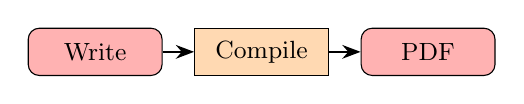
\begin{tikzpicture}[node distance=4mm]
        \node (a) [startstop] {Write};
        \node (b) [process, right=of a] {Compile};
        \node (c) [startstop, right=of b] {PDF};
        \draw [arrow] (a) -- (b);
        \draw [arrow] (b) -- (c);
      \end{tikzpicture}
      \end{center}
  \end{columns}
\end{frame}

% ═══ 26 — CODE, ALGORITHMS, PLOTS ════════════════════════════
\begin{frame}[fragile]{Code, Algorithms and Plots}
  \begin{columns}[T]
    \column{0.5\textwidth}
      \textbf{\small\texttt{listings}}: syntax highlighting for 80+ languages
      \begin{lstlisting}[language=Python]
def hello_world(name):
    """Greet someone by name."""
    print(f"Welcome, {name}!")

hello_world("Abel")
      \end{lstlisting}
    \column{0.46\textwidth}
      \begin{infobox}{softgreen}{\texttt{algorithm2e}}
        Numbered pseudocode with \texttt{\textbackslash KwIn}, \texttt{\textbackslash While},
        \texttt{\textbackslash Return}. The sample project has binary search.
      \end{infobox}
      \vspace{0.1cm}
      \begin{infobox}{royalblue}{\texttt{pgfplots}}
        Plots from formulas or data: lines, bars, even 3D surfaces. No Excel screenshots required.
      \end{infobox}
  \end{columns}
\end{frame}

% ═══ 27 — DIAGRAM GALLERY ════════════════════════════════════
\begin{frame}{The Diagram Gallery: 60+ Templates}
  \centering
  {\small Plain TikZ only, no heavy packages: copy, paste, edit the labels.}\\[0.2cm]
  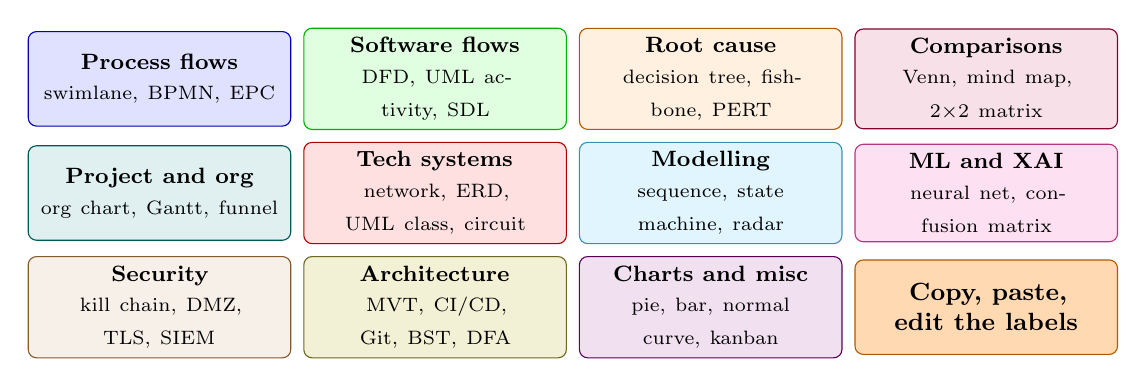
\begin{tikzpicture}
    \chip{0}{0}{blue}{Process flows}{swimlane, BPMN, EPC}
    \chip{3.5}{0}{green}{Software flows}{DFD, UML activity, SDL}
    \chip{7}{0}{orange}{Root cause}{decision tree, fishbone, PERT}
    \chip{10.5}{0}{purple}{Comparisons}{Venn, mind map, 2$\times$2 matrix}
    \chip{0}{-1.45}{teal}{Project and org}{org chart, Gantt, funnel}
    \chip{3.5}{-1.45}{red}{Tech systems}{network, ERD, UML class, circuit}
    \chip{7}{-1.45}{cyan}{Modelling}{sequence, state machine, radar}
    \chip{10.5}{-1.45}{magenta}{ML and XAI}{neural net, confusion matrix}
    \chip{0}{-2.9}{brown}{Security}{kill chain, DMZ, TLS, SIEM}
    \chip{3.5}{-2.9}{olive}{Architecture}{MVT, CI/CD, Git, BST, DFA}
    \chip{7}{-2.9}{violet}{Charts and misc}{pie, bar, normal curve, kanban}
    \node[chip=orange, fill=orange!30, font=\small\bfseries] at (10.5,-2.9)
      {Copy, paste,\\edit the labels};
  \end{tikzpicture}
\end{frame}

% ═══ 28 — DEMO: DIAGRAM GALLERY ══════════════════════════════
\demoslide{warmorange!80!midnightblue}{The Diagram Gallery}{Behold the Cheat Sheet}{%
  Open the Diagram Gallery file\\[0.15cm]
  \textbf{\color{accentyellow}Point out:} scroll the sections $\cdot$ copy the Cyber Kill Chain\\
  or the SIEM pipeline $\cdot$ change the labels $\cdot$ recompile}

% ═══ 29 — IMAGES UNDER CONTROL ═══════════════════════════════
\begin{frame}{Images Under Full Control}
  In Word, you drag and hope. In \LaTeX, you state the \emph{intent}.
  \vspace{0.2cm}
  \begin{columns}[T]
    \column{0.48\textwidth}
      \begin{infobox}{royalblue}{Text wrapping: \texttt{wrapfig}}
        Text flows naturally around an image placed left or right.
      \end{infobox}
      \vspace{0.1cm}
      \begin{infobox}{softgreen}{Side by side: \texttt{subcaption}}
        Aligned subfigures (a), (b) with one shared caption.
      \end{infobox}
    \column{0.48\textwidth}
      \begin{infobox}{warmorange}{Pin it: \texttt{float}}
        The \texttt{[H]} specifier anchors an image exactly where you wrote it.
      \end{infobox}
      \vspace{0.1cm}
      \begin{infobox}{lavender}{Clip it: TikZ}
        Crop an image into a circle, or put images inside flowchart nodes.
      \end{infobox}
  \end{columns}
\end{frame}

% ═══ 30 — TYPOGRAPHY SUPERPOWERS ═════════════════════════════
\begin{frame}{Typography Superpowers: What Word Can't Do}
  \begin{columns}[T]
    \column{0.56\textwidth}
      \begin{itemize}\small
        \item \textbf{Micro-typography} (\texttt{microtype}): protrusion and kerning, no ``rivers'' of white space
        \item \textbf{Exotic underlines} (\texttt{ulem}): \uwave{wavy}, \uuline{double}, \dashuline{dashed}, \dotuline{dotted}
        \item \textbf{Letter-spacing} (\texttt{soul}): \so{TRACKED HEADINGS}
        \item \textbf{Paragraph shapes} (\texttt{shapepar}): text filling a {\color{warmorange}\textbf{heart}} or {\color{royalblue}\textbf{diamond}}
        \item \textbf{Historical fonts} (\texttt{yfonts}): Fraktur, Gothic, Schwabacher
        \item \textbf{Also:} drop caps, outlined text, absolute placement
      \end{itemize}
    \column{0.4\textwidth}
      \begin{infobox}{royalblue}{Packages at a glance}
        \scriptsize
        \begin{tabular}{@{}ll@{}}
          \texttt{microtype} & kerning \\
          \texttt{soul}      & tracking \\
          \texttt{ulem}      & underlines \\
          \texttt{shapepar}  & shaped text \\
          \texttt{yfonts}    & blackletter \\
          \texttt{lettrine}  & drop caps \\
          \texttt{pdfrender} & outlined text \\
          \texttt{textpos}   & absolute position \\
        \end{tabular}
      \end{infobox}
      \vspace{0.1cm}
      \begin{funfact}
        \scriptsize All of these ship with Overleaf's TeX Live. Zero setup.
      \end{funfact}
  \end{columns}
\end{frame}

% ═══ 31 — DEMO: TYPOGRAPHY ═══════════════════════════════════
\demoslide{midnightblue!90!black}{Typography Superpowers}{Word Could Never}{%
  Open \texttt{advanced\_text\_formatting.tex} in Overleaf\\[0.15cm]
  \textbf{\color{accentyellow}Point out:} drop caps $\cdot$ sine-wave text $\cdot$ outlined text\\
  heart and diamond paragraphs $\cdot$ Fraktur $\cdot$ wavy and double underlines\\
  gradient boxes $\cdot$ drop shadow $\cdot$ dingbat bullets\\
  image wrapping $\cdot$ circular clipping $\cdot$ images inside flowchart nodes}

% ═══ 32 — PUSHING THE LIMITS ═════════════════════════════════
\begin{frame}{Pushing the Limits}
  If you can describe it mathematically or structurally, \LaTeX\ can typeset it:
  \vspace{0.1cm}
  \begin{columns}[T]
    \column{0.28\textwidth}
      \begin{center}
      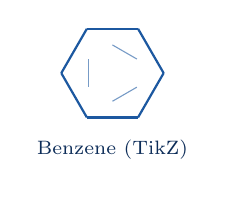
\begin{tikzpicture}[scale=0.65]
        \foreach \i in {0,1,2,3,4,5} {
          \draw[royalblue, thick] ({60*\i}:1) -- ({60*(\i+1)}:1);
        }
        \foreach \i in {0,2,4} {
          \draw[royalblue!60] ({60*\i+30}:0.55) -- ({60*\i+90}:0.55);
        }
        \node[font=\scriptsize, text=midnightblue] at (0,-1.5) {Benzene (TikZ)};
      \end{tikzpicture}
      \end{center}
    \column{0.40\textwidth}
      \begin{itemize}\footnotesize
        \item \textbf{Sheet music} --- \texttt{musixtex}
        \item \textbf{Chemistry} --- \texttt{chemfig}
        \item \textbf{Circuits} --- \texttt{circuitikz}
        \item \textbf{Chess} --- \texttt{skak}
        \item \textbf{QR codes} --- \texttt{qrcode}
        \item \textbf{Protocol headers} --- \texttt{bytefield}
        \item \textbf{Fractals, crosswords, Rubik's cubes} --- TikZ
      \end{itemize}
    \column{0.28\textwidth}
      \begin{quip}
        The question is never \textit{can \LaTeX\ do this?} It is only \textit{which package?}
      \end{quip}
      \vspace{0.1cm}
      \begin{cheatcode}
        \scriptsize Search CTAN (ctan.org) for any niche topic.
      \end{cheatcode}
  \end{columns}
\end{frame}

% ═══ 33 — DEBUGGING ══════════════════════════════════════════
\begin{frame}{How to Debug Like a Pro}
  \begin{columns}[T]
    \column{0.55\textwidth}
      \begin{itemize}\small
        \item When Overleaf flashes red, \textbf{don't panic.}
        \item Fix the \textbf{first} error: later ones are often side effects.
        \item Ignore the jargon. Find \texttt{l.42}: that's your broken line!
        \item \textbf{Undefined control sequence} $\rightarrow$ typo or missing package.
        \item \textbf{Missing \$ inserted} $\rightarrow$ math symbol outside math mode.
        \item \textbf{Runaway argument} $\rightarrow$ unmatched \texttt{\{}.
      \end{itemize}
    \column{0.42\textwidth}
      \begin{errorlog}
        ! Undefined control sequence.\\
        l.42 \textbackslash textbfs\{hello\}\\[0.2cm]
        ! Missing \$ inserted.\\
        l.67 E = mc\textasciicircum 2\\[0.2cm]
        $\rightarrow$ Fix: line 42 typo.
      \end{errorlog}
      \vspace{0.1cm}
      \begin{protip}
        Paste the red text into an AI assistant and ask for the fix. Still stuck? Comment out
        half the document with \texttt{\%} and bisect.
      \end{protip}
  \end{columns}
\end{frame}

% ═══ 34 — DEMO: LIVE DEBUGGING ═══════════════════════════════
\demoslide{codered!70!black}{Let's Break Things}{Live Debugging}{%
  \textbf{\color{accentyellow}Break on purpose:} misspell \texttt{\textbackslash textbf}\\
  delete a closing brace $\cdot$ use \texttt{\_} outside math\\
  Read the Logs panel, find the first error, fix it}

% ═══ 35 — HABITS ═════════════════════════════════════════════
\begin{frame}{Habits of Happy \LaTeX\ Users}
  \begin{columns}[T]
    \column{0.5\textwidth}
      \begin{itemize}\small
        \item Use \textbf{semantic commands}: \texttt{\textbackslash emph}, \texttt{\textbackslash section}.
        \item Define repeated formatting once with \texttt{\textbackslash newcommand}.
        \item Always \texttt{\textbackslash label} and \texttt{\textbackslash ref}; never type numbers.
        \item Compile often: small errors are easy to find.
      \end{itemize}
    \column{0.47\textwidth}
      \begin{itemize}\small
        \item One idea per source line, with \texttt{\%} comments marking sections.
        \item Keep figures in \texttt{figures/} and set \texttt{\textbackslash graphicspath}.
        \item Never use \texttt{\textbackslash\textbackslash} for vertical space between paragraphs.
        \item Let AI help, then \textbf{verify} that it compiles.
      \end{itemize}
  \end{columns}
  \vspace{0.3cm}
  \begin{quip}
    Write the content. Let \LaTeX\ handle the design.
  \end{quip}
\end{frame}

% ═══ 36 — THE FINAL REVEAL ═══════════════════════════════════
\begin{frame}{Start Building...}
  \begin{itemize}
    \item Go to \textbf{Overleaf.com} and sign up for a free account.
    \item Open the \textbf{Sample Project} to explore the code.
    \item Use the \textbf{Study Guide} and the \textbf{Diagram Gallery} (60+ templates).
    \item Browse \texttt{advanced\_text\_formatting.tex} when you want to show off.
    \item Never fight MS (Microsoft) Word over a serious technical report again.
  \end{itemize}
  \vspace{0.3cm}
  \pause
  \begin{tcolorbox}[enhanced, colback=midnightblue, colframe=warmorange,
      colbacktitle=warmorange, coltitle=midnightblue,
      arc=8pt, boxrule=2pt, fonttitle=\large\bfseries,
      title={One more thing...}]
    \begin{center}
      {\color{white}
      This entire slide deck wasn't made in PowerPoint.\\[0.2cm]
      I coded it in \LaTeX\ using the \texttt{\color{accentyellow}beamer} package.\\[0.2cm]
      \textit{\color{white!75}These slides ARE the demo.}}
    \end{center}
  \end{tcolorbox}
\end{frame}

\end{document}
